\documentclass[]{scrartcl}

\usepackage[utf8]{inputenc}
\usepackage{amsmath,amssymb}
\usepackage{xcolor}
\usepackage{seqsplit} % splitting long seqs 
\usepackage{fontawesome} % cool icons
\usepackage{cmbright} % better fonts
\usepackage[most]{tcolorbox}
\usetikzlibrary{shapes.geometric}
\usepackage{scrlayer-scrpage}
\usepackage{xcolor}
\usepackage[section]{placeins}
\usepackage{listings}
\usepackage{longtable}
\usepackage{url}

\definecolor{plusgreen}{RGB}{17,87,64}
\newcommand{\ZZ}{\mathbb{Z}}


%%% exercise text formatting code - DO NOT CHANGE
\newcounter{exercise}
\newcounter{qid}[section]
\newcommand{\exerciseprefix}{prefix}
\newcommand{\questiontitle}{Questions}
\newcommand{\blockid}{B3}
\newcommand{\exname}{}
\newtcolorbox{exercisebox}[2][]{%
  colback=gray!5,
  colframe=plusgreen,
  fonttitle=\bfseries,
  title={\questiontitle},
  breakable,
  enhanced,
  sharp corners,
  boxrule=0.5pt,
  %before upper=\refstepcounter{exercise},
  overlay unbroken and last ={%
    % only draw points at end of box
    \if\relax\detokenize{#2}\relax\else
        \node[draw,ellipse,fill=orange,inner xsep=6pt, inner ysep=2pt,font=\small]
        at ([yshift=-2pt]frame.south) {#2 pts};
    \fi
  },
  #1
}



\lstdefinestyle{plusStyle}{
    basicstyle=\ttfamily\small,
    % --- Green Elements ---
    frame=single,
    rulecolor=\color{plusgreen},       % Frame border color
    numbers=left,
    numberstyle=\tiny\color{plusgreen}, % Line number color
    % ----------------------
    stepnumber=1,
    numbersep=8pt,
    breaklines=true,
    breakatwhitespace=false,
    postbreak=\mbox{\textcolor{plusgreen}{$\hookrightarrow$}\space}, % Green wrap arrow
    showstringspaces=false
}



\lstdefinestyle{sageStyle}{
    basicstyle=\ttfamily\small,
    frame=single,
    rulecolor=\color{plusgreen},
    numbers=left,
    numberstyle=\tiny\color{plusgreen},
    stepnumber=1,
    numbersep=8pt,
    breaklines=true,
    breakatwhitespace=false,
    postbreak=\mbox{\textcolor{plusgreen}{$\hookrightarrow$}\space},
    showstringspaces=false,
    language=Python,
    keywordstyle=\color{plusgreen}\bfseries,
    commentstyle=\color{gray}\itshape,
    stringstyle=\color{orange},
    morekeywords={matrix,vector,Zmod,print,range,list,len,ord,chr,pow,append,extend}
}




\newcommand{\ctone}{CrypTool1}
\newcommand{\cttwo}{CrypTool2}
\newcommand{\ctonline}{CrypToolOnline}
\newcommand{\yoursolutionhere}{\textbf{YOUR-SOLUTION-HERE}}
\newcommand{\filename}[1]{\texttt{#1}}


\title{Homework Exercise Sheet 3\\Introduction to Cryptography \& IT-Security\\PS 511.088\\Summer Semester 2026}



%%%%%%%%%%%%%%%%%%%%%%%%%%%%%%%%%%%%%%%%%%%%%
% DO NOT MODIFY ANYTHING BEFORE THIS LINE IN THIS FILE %%%%%%%%%%%%
%%%%%%%%%%%%%%%%%%%%%%%%%%%%%%%%%%%%%%%%%%%%%%%%%%%%%%%%%%%%%%%%%
%%%%%%%%%%%% USE GROUP NAME FROM BLACKBOARD BELOW AND NO PERSONAL IDENTIFIABLE INFORMATION %%%%%%%%%%%%%%%%%%
\newcommand{\groupname}{Malware Hunters}
\author{\groupname}
%%%%%%%%%%%%%%%%%%%%%%%%%%%%%%%%%%%%%%%%%%%%%%%%%%%%%%%%%%%%%%%%%%%%%%%%%%


% format pagestyle below
\clearpairofpagestyles
%% Header
\chead{{\small \groupname}} %adjust font size as needed
%% Footer
\ifoot{{\small D. Simos, B. Garn, D. Schreiber}}
\cfoot{{\small University of Salzburg}}
\ofoot{{\small PS 511.088 SS2026}}
\pagestyle{scrheadings}


%%%%%%%%%%%%%%%%%
\begin{document}
\maketitle
\abstract{This is the third homework exercise sheet for the proseminar \emph{Introduction to Cryptography and IT-Security} (PS 511.088) covering the block \emph{Classical Cryptography and Secure Protocols} to be completed before the proseminar on May 20, 2026 with a maximum of 20 points to be achieved. Submission deadline in Blackboard is May 19, 2026 at 12:59 PM. Late submissions will \textbf{not} be graded.

Use CrypTool software and/or SAGE to assist you in solving the exercises and the provided \LaTeX~code in the appendix to format your report, using the source \LaTeX~of the homework exercise sheet. Submit both resulting \texttt{tex/pdf} files in Blackboard. No other format is allowed.}
\date{}

\pagebreak




\stepcounter{exercise}
\pagebreak
\renewcommand{\exname}{Matrix-based Cryptosystems: Hill Cipher}
\section*{PS-\blockid{}-E\theexercise: \exname{}}
Matrix-based crypto systems provide structure, where resulting structural properties can be taken advance of by both the user of such a system as well as by an adversary attacking such a system. In this exercise, we consider the Hill cipher. For more details in the mechanics and the underlying structure of the Hill cipher, please see: \url{https://caesarcipher.org/ciphers/hill}



\stepcounter{qid}
\renewcommand{\exerciseprefix}{PS-\blockid{}-E\theexercise: \exname-Q\theqid}
\renewcommand{\questiontitle}{\exerciseprefix{}: Encryption/Decryption in CTO}
\begin{exercisebox}{0.1}
Use CTO to (\url{https://legacy.cryptool.org/en/cto/hill}) to encrypt the following statement
\begin{quote}
    THISTEXTSHOULDREMAINSECRET
\end{quote}
using the key
\begin{equation} 
    \begin{pmatrix}
    23 & 10 \\
     0 &  9
     \end{pmatrix}
\end{equation}
Decrypt it also again. Document all performed steps.  
\end{exercisebox}

\paragraph{Answer:}

We navigated to \url{https://legacy.cryptool.org/en/cto/hill} and performed the following steps:

\begin{enumerate}
    \item \textbf{Setup}: Selected alphabet size 26 (A--Z) and key size $2\times2$.
    \item \textbf{Key entry}: Entered the key matrix entries $k_{11}=23$, $k_{12}=10$, $k_{21}=0$, $k_{22}=9$.
    \item \textbf{Encryption}: Entered the plaintext \texttt{THISTEXTSHOULDREMAINSECRET} (26 characters, forming 13 blocks of length~2) and clicked \emph{Encrypt}.
    \item \textbf{Result}: CTO produced the ciphertext \texttt{NLAGJKRPQLCYXBPKQACNMKIXWP}.
    \item \textbf{Decryption}: Pasted the ciphertext back, clicked \emph{Decrypt}, and recovered \texttt{THISTEXTSHOULDREMAINSECRET}. $\checkmark$
\end{enumerate}

\medskip
\begin{center}
\begin{tabular}{|l|l|}
\hline
\textbf{Plaintext}  & \texttt{THISTEXTSHOULDREMAINSECRET} \\
\hline
\textbf{Ciphertext} & \texttt{NLAGJKRPQLCYXBPKQACNMKIXWP} \\
\hline
\textbf{Decrypted}  & \texttt{THISTEXTSHOULDREMAINSECRET} \\
\hline
\end{tabular}
\end{center}

\textbf{Manual verification of the first block} (\texttt{TH} $\to$ numerics $19,7$):
\[
\begin{pmatrix}23 & 10\\0 & 9\end{pmatrix}\begin{pmatrix}19\\7\end{pmatrix}
=\begin{pmatrix}23\cdot19+10\cdot7\\0\cdot19+9\cdot7\end{pmatrix}
=\begin{pmatrix}507\\63\end{pmatrix}
\equiv\begin{pmatrix}507\bmod26\\63\bmod26\end{pmatrix}
=\begin{pmatrix}13\\11\end{pmatrix}
\;\longrightarrow\;\texttt{NL}\checkmark
\]


\stepcounter{qid}
\renewcommand{\exerciseprefix}{PS-\blockid{}-E\theexercise: \exname-Q\theqid}
\renewcommand{\questiontitle}{\exerciseprefix{}: Encryption/Decryption in Sage}
\begin{exercisebox}{0.9}
Use the same key as in the previous question and perform the corresponding encryption/decryption again using Sage. Use Sage-functionality to implement your solution (e.g., for matrix-vector multiplication). 
\end{exercisebox}

\paragraph{Answer:}

The following SageMath code performs encryption and decryption of the plaintext over $\mathbb{Z}_{26}$:

\begin{lstlisting}[style=sageStyle, caption={Hill cipher encryption and decryption in SageMath}]
R = Zmod(26)

# Key matrix K
K = matrix(R, [[23, 10], [0, 9]])

# Helper functions
def str_to_nums(s):
    return [ord(c) - ord('A') for c in s]

def nums_to_str(lst):
    return ''.join(chr(int(n) % 26 + ord('A')) for n in lst)

# Encrypt
plaintext = "THISTEXTSHOULDREMAINSECRET"
nums = str_to_nums(plaintext)

cipher_nums = []
for i in range(0, len(nums), 2):
    block = vector(R, [nums[i], nums[i+1]])
    enc = K * block
    cipher_nums += list(enc)

ciphertext = nums_to_str(cipher_nums)
print("Ciphertext:", ciphertext)
# Output: NLAGJKRPQLCYXBPKQACNMKIXWP

# Decrypt using K^{-1} mod 26
K_inv = K^(-1)
print("K inverse:", K_inv)
# det(K) = 23*9 - 10*0 = 207 = 25 (mod 26), inverse of 25 is 25
# K^{-1} = 25 * [[9,-10],[0,23]] mod 26 = [[17,10],[0,3]]

dec_nums = []
for i in range(0, len(cipher_nums), 2):
    block = vector(R, [cipher_nums[i], cipher_nums[i+1]])
    dec = K_inv * block
    dec_nums += list(dec)

decrypted = nums_to_str(dec_nums)
print("Decrypted:", decrypted)
# Output: THISTEXTSHOULDREMAINSECRET
\end{lstlisting}

\textbf{Results:}

The determinant is $\det(K) = 23 \cdot 9 - 10 \cdot 0 = 207 \equiv 25 \pmod{26}$. Since $\gcd(25,26)=1$, the matrix is invertible. The modular inverse of $25$ modulo $26$ is $25$ (since $25 \cdot 25 = 625 = 24\cdot 26 + 1 \equiv 1$). Hence:
\[
K^{-1} = 25 \cdot \begin{pmatrix}9 & -10 \\ 0 & 23\end{pmatrix} \equiv \begin{pmatrix}17 & 10 \\ 0 & 3\end{pmatrix} \pmod{26}
\]

\begin{center}
\begin{tabular}{|l|l|}
\hline
\textbf{Ciphertext (Sage)} & \texttt{NLAGJKRPQLCYXBPKQACNMKIXWP} \\
\hline
\textbf{Decrypted (Sage)}  & \texttt{THISTEXTSHOULDREMAINSECRET} $\checkmark$ \\
\hline
\end{tabular}
\end{center}

\stepcounter{qid}
\renewcommand{\questiontitle}{Preparation (!) for question PS-\blockid{}-E\theexercise-Q-\theqid}
\begin{exercisebox}{}
Download from Blackboard and work with the file \filename{blockIII\_Hill\_KPApairs.sage}. This file contains SageMath statements that you can directly use for solving question PS-\blockid{}-E\theexercise-Q-\theqid. 
\end{exercisebox}

\renewcommand{\exerciseprefix}{PS-\blockid{}-E\theexercise: \exname-Q\theqid}
\renewcommand{\questiontitle}{\exerciseprefix{}: Known-plaintext attack}
\begin{exercisebox}{4}
Perform a known-plaintext attack against the Hill cipher given that you have - somehow - obtained the plaintext-ciphertext pairs given in the file \filename{blockIII\_Hill\_KPApairs.sage}. The goal is to recover the key. 

{\small
Guidance:
\begin{enumerate}
    \item Determine the dimensions of the matrix $K$ representing the key. 
    \item Write the known-pairs as $KP=C$; with appropriate matrices $P$ for the plaintext (known at this point from KPA input), $K$ for the key (still unknown at this point) and $C$ for the ciphertext (known at this point from KPA input). Pay attention that corresponding columns in the matrices $P$ and $C$ appear in the same order. 
    \item Find a maximal - according to set inclusion relation - linear independent set of plaintext-columns within $P$ called $P^{\prime}$.
    \item Select corresponding sub-matrix $C^{\prime}$ of $C$. 
    \item Compute the inverse of $P^{\prime}$.
    \item Obtain the key $K$ as result of computing $C^{\prime} \cdot (P^{\prime})^{-1}$. 
\end{enumerate}

}
\end{exercisebox}

\paragraph{Answer:}

We loaded \filename{blockIII\_Hill\_KPApairs.sage} which provides 20 plaintext--ciphertext column-vector pairs over $\mathbb{Z}_{64}$. Each vector has \textbf{10 components}.

\medskip
\noindent\textbf{Step 1: Key matrix dimensions.}

Since each plaintext/ciphertext vector has 10 entries, the Hill cipher equation $\mathbf{c} = K\mathbf{p}$ implies $K \in (\mathbb{Z}_{64})^{10\times 10}$.

\medskip
\noindent\textbf{Step 2: Matrix equation.}

Stacking all 20 column-vector pairs side by side gives
\[
K \cdot P = C \pmod{64},
\]
where $P,C \in (\mathbb{Z}_{64})^{10\times 20}$ with each column being one plaintext/ciphertext vector respectively.

\medskip
\noindent\textbf{Step 3: Maximal linearly independent set $P'$.}

Applying modular Gaussian elimination over $\mathbb{Z}_{64}$ to the columns of $P$, we identify the following 10 columns (0-indexed) as a maximal linearly independent set:
\[
\text{Independent column indices: } \{0,\;1,\;3,\;7,\;9,\;12,\;13,\;16,\;18,\;19\}.
\]
These 10 columns form the $10\times 10$ submatrix $P'$.

\medskip
\noindent\textbf{Step 4: Corresponding ciphertext submatrix $C'$.}

We select the same columns from $C$ to obtain $C' \in (\mathbb{Z}_{64})^{10\times 10}$.

\medskip
\noindent\textbf{Step 5: Inverse of $P'$.}

We compute $(P')^{-1} \pmod{64}$ via modular Gaussian elimination. Verification: $P' \cdot (P')^{-1} \equiv I_{10} \pmod{64}$. $\checkmark$

\medskip
\noindent\textbf{Step 6: Key recovery.}

\[
K = C' \cdot (P')^{-1} \pmod{64}.
\]

\textbf{Recovered key matrix $K \in (\mathbb{Z}_{64})^{10\times10}$:}
\[
K =
\begin{pmatrix}
 2 & 52 & 52 & 30 & 23 & 49 &  7 & 59 &  9 & 27 \\
22 & 21 &  8 & 29 & 55 &  5 & 36 & 60 & 13 & 29 \\
44 & 11 &  6 & 54 & 21 & 25 & 42 &  6 &  5 & 34 \\
22 & 36 & 28 & 19 &  8 & 40 &  5 & 60 & 47 & 24 \\
 7 & 57 & 55 & 46 &  9 & 26 & 18 & 56 &  6 & 10 \\
48 & 54 & 49 & 60 & 59 & 33 &  7 & 37 & 34 & 39 \\
20 &  5 &  7 & 22 & 38 & 21 & 56 & 24 &  4 & 24 \\
30 & 29 &  3 & 14 & 24 & 18 & 13 & 19 & 31 & 23 \\
36 & 13 & 57 & 58 & 27 & 42 & 45 & 29 & 50 &  3 \\
62 & 27 & 58 & 31 & 15 & 51 & 63 & 39 &  1 & 30
\end{pmatrix}
\pmod{64}
\]

\textbf{Verification:} Applying $K$ to all 20 plaintext vectors reproduces the corresponding ciphertext vectors modulo~64 for every pair. $\checkmark$

\medskip
The SageMath code used:

\begin{lstlisting}[style=sageStyle, caption={Known-plaintext attack on Hill cipher over $\mathbb{Z}_{64}$}]
# After: load('blockIII_Hill_KPApairs.sage')
# KPApairs is a list of 20 (plaintext_col, ciphertext_col) matrix pairs

R = Zmod(64)

# Step 2: Build 10x20 plaintext and ciphertext matrices
P = matrix(R, [[KPApairs[j][0][i,0] for j in range(20)] for i in range(10)])
C = matrix(R, [[KPApairs[j][1][i,0] for j in range(20)] for i in range(10)])

# Step 3 & 4: Select 10 linearly independent columns (found via echelon form)
indep = [0, 1, 3, 7, 9, 12, 13, 16, 18, 19]
P_prime = P.matrix_from_columns(indep)
C_prime = C.matrix_from_columns(indep)

# Step 5: Compute inverse of P'
P_prime_inv = P_prime^(-1)

# Step 6: Recover the key
K = C_prime * P_prime_inv
print("Recovered key K =")
print(K)

# Verification: K*P should equal C (mod 64)
assert K * P == C
print("All 20 KPA pairs verified successfully!")
\end{lstlisting}


\stepcounter{qid}
\renewcommand{\exerciseprefix}{PS-\blockid{}-E\theexercise: \exname-Q\theqid}
\renewcommand{\questiontitle}{\exerciseprefix{}: Chosen-plaintext attack}
\begin{exercisebox}{1}
Consider a chosen-plaintext attack on the Hill cipher. For a positive natural number $n$, show that for given key matrix dimension $n \times n$, you can obtain the key with $n$ queries. Argue further why $n$ is an exact number, in the sense that fewer queries are insufficient and strictly more queries not necessary. 

\end{exercisebox}

\paragraph{Answer:}

\textbf{Construction with $n$ queries.}
Choose the $n$ standard basis vectors as the $n$ plaintexts:
\[
\mathbf{e}_1 = (1,0,\ldots,0)^\top,\quad
\mathbf{e}_2 = (0,1,0,\ldots,0)^\top,\quad \ldots,\quad
\mathbf{e}_n = (0,\ldots,0,1)^\top.
\]
Querying the encryption oracle on each $\mathbf{e}_i$ yields the ciphertext
\[
\mathbf{c}_i = K\,\mathbf{e}_i = K_{\bullet,\,i},
\]
i.e.\ exactly the $i$-th column of $K$. Hence $n$ queries reveal all $n$ columns and $K$ is fully recovered. More formally, stacking the responses gives $C = K\cdot I_n$, so $K = C\cdot I_n^{-1} = C$.

\medskip
\textbf{Why fewer than $n$ queries are insufficient.}
With only $k < n$ queries we learn at most $k$ columns of $K$. The remaining $n-k$ columns are completely unconstrained by the observed query--response pairs: for any choice of values for those columns the encryption of the $k$ chosen plaintexts is unchanged. Hence the key cannot be uniquely determined from fewer than $n$ queries.

\medskip
\textbf{Why more than $n$ queries are unnecessary.}
Once we have queried all $n$ basis vectors we have recovered all $n^2$ entries of $K$. Any additional query provides only information that is already deducible from $K$, i.e.\ it is redundant. Therefore strictly more than $n$ queries are not needed.

\medskip
\textbf{Conclusion.} The exact query complexity of the chosen-plaintext attack against an $n\times n$ Hill cipher is $\mathbf{n}$: sufficient to recover $K$ completely, and necessary since any $k<n$ queries leave at least one column undetermined.


\pagebreak
\stepcounter{exercise}
\renewcommand{\exname}{Vigen\`ere Cipher}
\section*{PS-\blockid{}-E\theexercise: \exname{}}
A poly-alphabetic substitution cipher uses multiple simple substitutions
to encrypt a message. The Vigen\`ere cipher is a classic poly-alphabetic
substitution cipher, where its main purpose  is to distribute the frequencies so that the
characters in the ciphertext are all likely to occur around the same number
of times. For more details in the mechanics and the underlying structure of the Vigen\`ere cipher, please see: \url{https://caesarcipher.org/ciphers/vigenere}
\stepcounter{qid}
\renewcommand{\exerciseprefix}{PS-\blockid{}-E\theexercise: \exname-Q\theqid}
\renewcommand{\questiontitle}{\exerciseprefix{}: Attack using Frequency Analysis}
\begin{exercisebox}{6}
Suppose that the following ciphertext was created using a
Vigen\`ere cipher (blank spaces are not encrypted):
\begin{quote}
\texttt{\seqsplit{GZE AKA VK WNLCUANT QOH JITZT AGW OMT QGNG OOEJY GZEL SRR LOB TUFQ DRUICZEEANT QOHJ GEGUC HRRKEALAGAOA KLVVEF LO AGTVUE GZIF EEFKATW
PEGFRKSBJ SZATU KALK TUST IAGRFEEW IF MNOJENCAODE OMT UW FBJGBL TB LEYD YBM AOGUG XRRIURFCL SNNDYFAS NFD XSSVKKV LEFLS NJE PGMVFG NFD LGUE YRBMP FLIYD HNKNG XIAASUWD GZE OWAZWR FDIQWS
GZE FWCEWT CSSFOOEV TB LHR MNVNEEKIGQ WVXI VK PNKSJGRQ GNR LWB LHEWE SGUE XIIW SVP SRNEA WITZT AANR REEG BHL SUZH QGNG LEYD AAQOAW EFHEPAAYDY AGT GZE VL DRHAELMRFT
VX YBM AEW RRSDVFG GZIF QOH SRR HRBTAODY N URLHTBYRNHHL KTHVEAL OE SN AKA NYEAL TEQIAY TB JEPJUVL YBMR TJOHH FBJ A GGP FWCEWT ZASFAOA ANIGLIANT HIMRA NFD SJER UOSXER
JEZWMOWR GZAG LHR TEFL WNQ TB ZIQW A ZWSFSGR AS GG PHL IG AN LGUE 
HRRKEALAGAOA TEPSUFW NBTOQQ RRSDF LHR XIAW PEANG SNLOAL LHR UIN GNPW LBKT N EEFKATW IA S TJWEG SBBMT CAZMS
TUW VVYEAWRR UICZEE AS YAKR S CNWSNJ SNDAQ TUG OIGZ MBJE YWTGMCR SNQ DEFK DEWSFANT SNQ SLFG IG MSRK A XWYJGRQ LHNL YBMR TJOHH PEGBNTLL XOEYOG LO NYRRW OA
TY GZE JSY GZE UADQWN ZWSFSGR AN GZIF LEKL IF ST GZE IWRL WNQ TUG QOH ZAIW TB VEPAPUWR VL FVJSG LO SANQ GUG OHNL YBMR AWXG SSFAGAEEAL WVDL OW
TUW NFS HNK A OSCXVOBJ IA QOHJ LNHTBH BHL IG GNYQ APLIISTRK WUWN LGU BHEA HOJWRCGIAL SB TE PSRRXUY OIGZ YBMR CJEFWNGSTVGN FCIYDS BJ TUWY JALY CNBO
CEQPGGGESPUQ IF WAFQ UALIY QOH JENDIMW TUST RNEEQ GEGUC AN PDAFK IF MSVFG GZE FSMR CELOOEV WUACU AS CJOOSBYQ TUW NNEE BX TUW CBXFRW SUGP AWXG VOBJ
HVVDRF MRKSNYE FLAEL YBMR AWXG SSFAGAEEAL IF LO PJAPC TUAS PAPUWR NFD CJEFWNG ZOJ QOH VIQ AT VF FVNE ZANHLEF GR YWSF FEKL TVEE UADQWN ZWSFSGR WNQ.}}
\end{quote}
Perform a cryptanalysis of this ciphertext and consider the following:
\begin{enumerate}
    \item What keyword length has been used? (2 points)
    \item Use \url{https://legacy.cryptool.org/en/cto/vigenerebreak} functionality of CrypTool-Online to decrypt the ciphertext provided above. (4 points)
\end{enumerate}
\end{exercisebox}

\paragraph{Answer:}

\textbf{1. What keyword length has been used?}

Repeated ciphertext fragments such as GZE QOH


appear multiple times in the ciphertext. The distances between repeated
occurrences are:

\begin{verbatim}
GZE : 39, 210, 15, 120, 417, 6, 30, 255
QOH : 48, 354, 432, 81, 123, 165
\end{verbatim}

Computing the greatest common divisor (GCD) of these distances gives:

\[
\gcd(39,210,15,120,417,6,30,255)=3
\]

and

\[
\gcd(48,354,432,81,123,165)=3
\]

Therefore, the most likely keyword length is:3


\bigskip

\textbf{2. Use CrypTool-Online functionality to decrypt the ciphertext.}

Using the CrypTool Online Vigen\`ere Break functionality and
frequency analysis, the recovered keyword is:

\begin{center}
\texttt{NSA}
\end{center}

Using the recovered keyword NSA, the ciphertext was successfully
decrypted. The plaintext is:

\begin{lstlisting}[breaklines=true,
                   basicstyle=\ttfamily\scriptsize,
                   columns=fullflexible,
                   frame=single]
THE NSA IS WATCHING YOU RIGHT NOW BUT DONT WORRY THEY ARE TOO BUSY
DECIPHERING YOUR GROUP PRESENTATION SLIDES TO NOTICE THIS MESSAGE
PROFESSOR SMITH SAYS THAT VIGENERE IS UNBREAKABLE BUT HE FORGOT TO
TELL YOU ABOUT FREQUENCY ANALYSIS AND KASISKI TESTS ARE COMING AND
YOUR GROUP STILL HASNT FINISHED THE BEAMER SLIDES

THE SECRET PASSWORD TO THE UNIVERSITY WIFI IS PASSWORD ONE TWO THREE
FOUR FIVE SIX SEVEN EIGHT NINE ZERO BUT SHHH DONT TELL ANYONE
ESPECIALLY NOT THE IT DEPARTMENT

IF YOU ARE READING THIS YOU ARE PROBABLY A CRYPTOGRAPHY STUDENT OR
AN NSA AGENT TRYING TO RECRUIT YOUR GROUP FOR A TOP SECRET MISSION
INVOLVING PIZZA AND FREE COFFEE

REMEMBER THAT THE BEST WAY TO HIDE A MESSAGE IS TO PUT IT IN YOUR
PRESENTATION BECAUSE NOBODY READS THE FINE PRINT ANYWAY

THE CIA ONCE LOST A MESSAGE IN A TWEET ABOUT PIZZA THE VIGENERE
CIPHER IS LIKE A CAESAR SALAD BUT WITH MORE LETTUCE AND LESS
DRESSING AND ALSO IT USES A KEYWORD THAT YOUR GROUP PROBABLY
FORGOT TO AGREE ON

BY THE WAY THE HIDDEN MESSAGE IN THIS TEXT IS AT THE VERY END BUT
YOU HAVE TO DECIPHER IT FIRST TO FIND OUT WHAT YOUR NEXT ASSIGNMENT
WILL BE

THE NSA HAS A BACKDOOR IN YOUR LAPTOP BUT IT ONLY ACTIVATES WHEN
YOU OPEN POWERPOINT SO BE CAREFUL WITH YOUR PRESENTATION SKILLS OR
THEY WILL KNOW

CRYPTOGRAPHY IS EASY UNTIL YOU REALIZE THAT EVERY GROUP IN CLASS IS
USING THE SAME KEYWORD WHICH IS PROBABLY THE NAME OF THE COFFEE
SHOP NEXT DOOR

HIDDEN MESSAGE START YOUR NEXT ASSIGNMENT IS TO CRACK THIS CIPHER
AND PRESENT HOW YOU DID IT IN FIVE MINUTES OR LESS NEXT TIME
HIDDEN MESSAGE END
\end{lstlisting}

\pagebreak
\stepcounter{exercise}
\renewcommand{\exname}{DES}
\section*{PS-\blockid{}-E\theexercise: DES}
The \emph{data encryption standard} has been used widely in the past, but is considered a legacy cryptosystem today. In particular, it is NOT (!) considered \emph{secure} anymore! However, both its design as well as its modes of operation still provide valuable insights into cryptographic design even today from an educational perspective. For this exercise, please make use of the Avalanche (DES) template in CrypTool 2 to assist you. 


\stepcounter{qid}
\renewcommand{\exerciseprefix}{PS-\blockid{}-E\theexercise: \exname-Q\theqid}
\renewcommand{\questiontitle}{\exerciseprefix{}: Mechanics of bit manipulation in DES}
\begin{exercisebox}{4}
\begin{itemize}
 \item  What is the output of the first round of the DES algorithm when the plaintext
and the key are both all zeros?
 \item  What is the output of the first round of the DES algorithm when the plaintext
and the key are both all ones?
\end{itemize}

\end{exercisebox}

\paragraph{Answer:} In the both scenarios, both the intial and modified message are the same. No bits were flipped.

\begin{figure}[h]
    \centering
    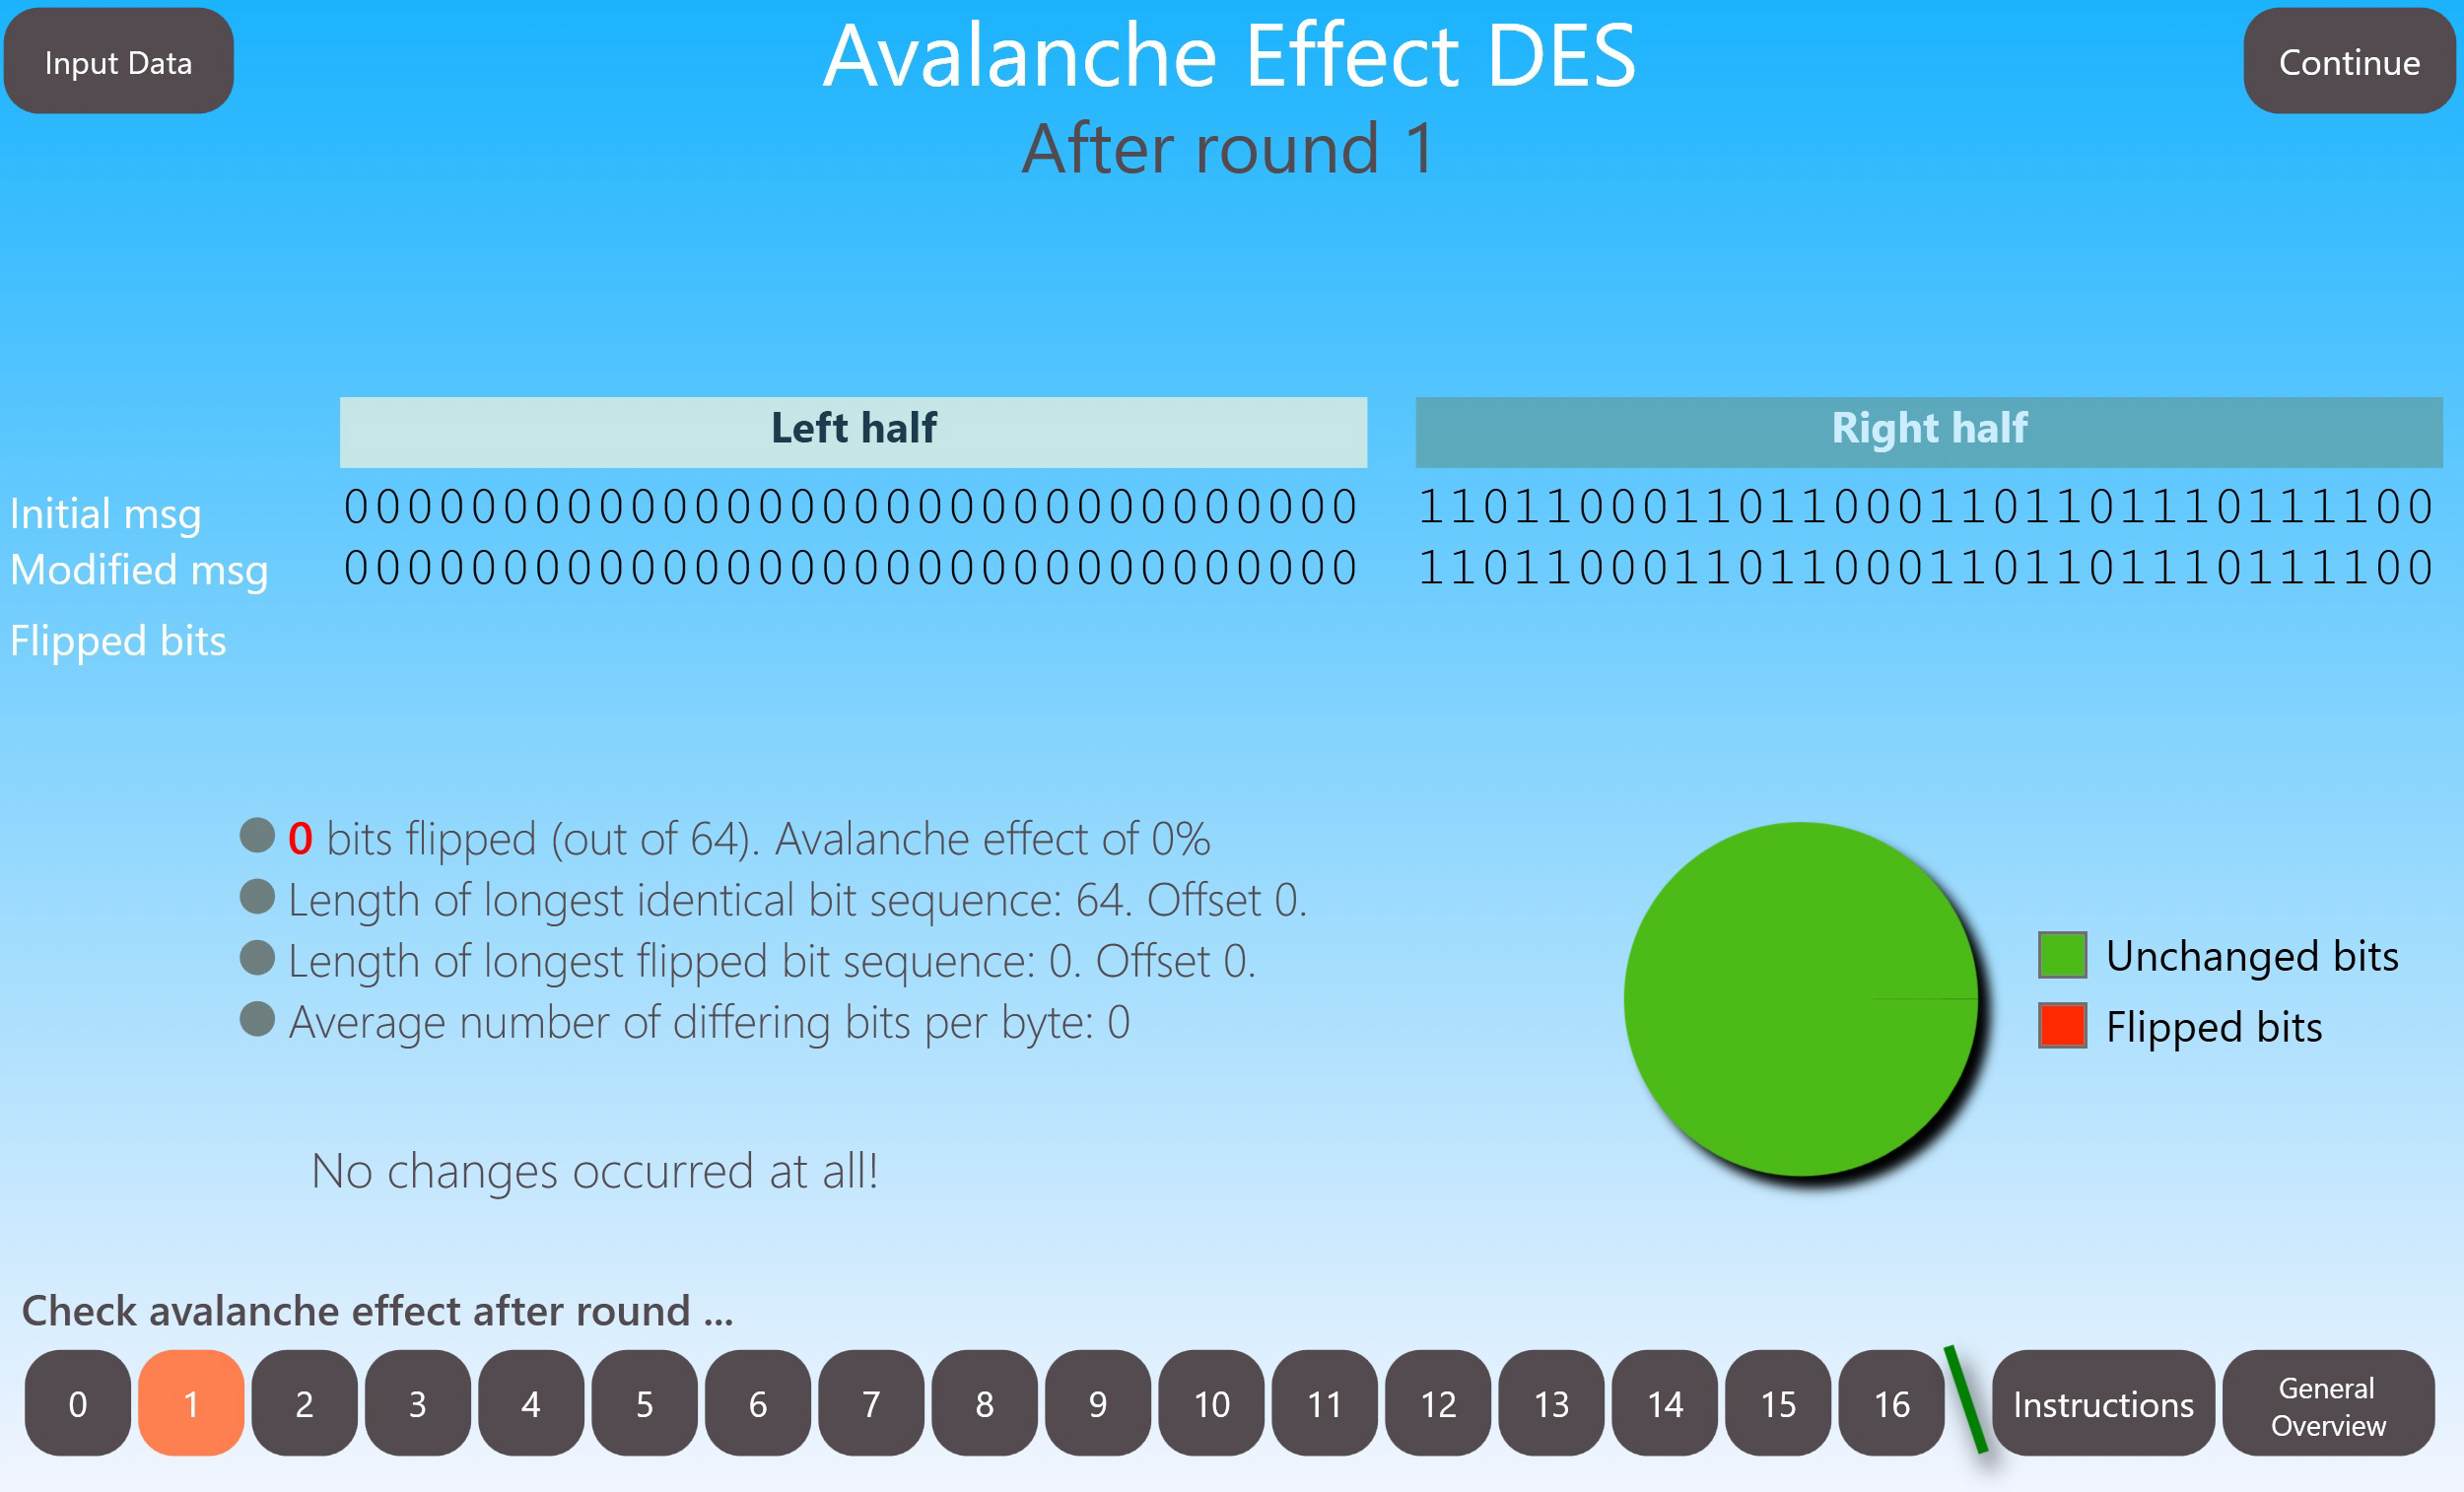
\includegraphics[scale=0.1]{image copy.png}
    \caption{DES Avalanche Effect Results}
    \label{fig:des-avalanche}
\end{figure}
\stepcounter{qid}
\renewcommand{\exerciseprefix}{PS-\blockid{}-E\theexercise: \exname-Q\theqid}
\renewcommand{\questiontitle}{\exerciseprefix{}: Avalanche effect in DES}
\begin{exercisebox}{4}
Remember that it is desirable for good block ciphers that a change in one input
bit affects many output bits, a property that is called diffusion or the avalanche
effect. We try now to get a feeling for the avalanche property of DES. We apply an
input word that has a “1” at bit position 57 and all other bits as well as the key are
zero. (Note that the input word has to run through the initial permutation.)
\begin{enumerate}
\item What is the output after the first round?
\item How many output bit after the first round have actually changed compared to
the case when the plaintext is all zero? (Observe that we only consider a single
round here. There will be more and more output differences after every new
round. Hence the term avalanche effect.)
\end{enumerate}
\end{exercisebox}

\paragraph{Answer:} As seen on the photo, the total number of output bits changed is 6. 

\begin{figure}[h]
    \centering
    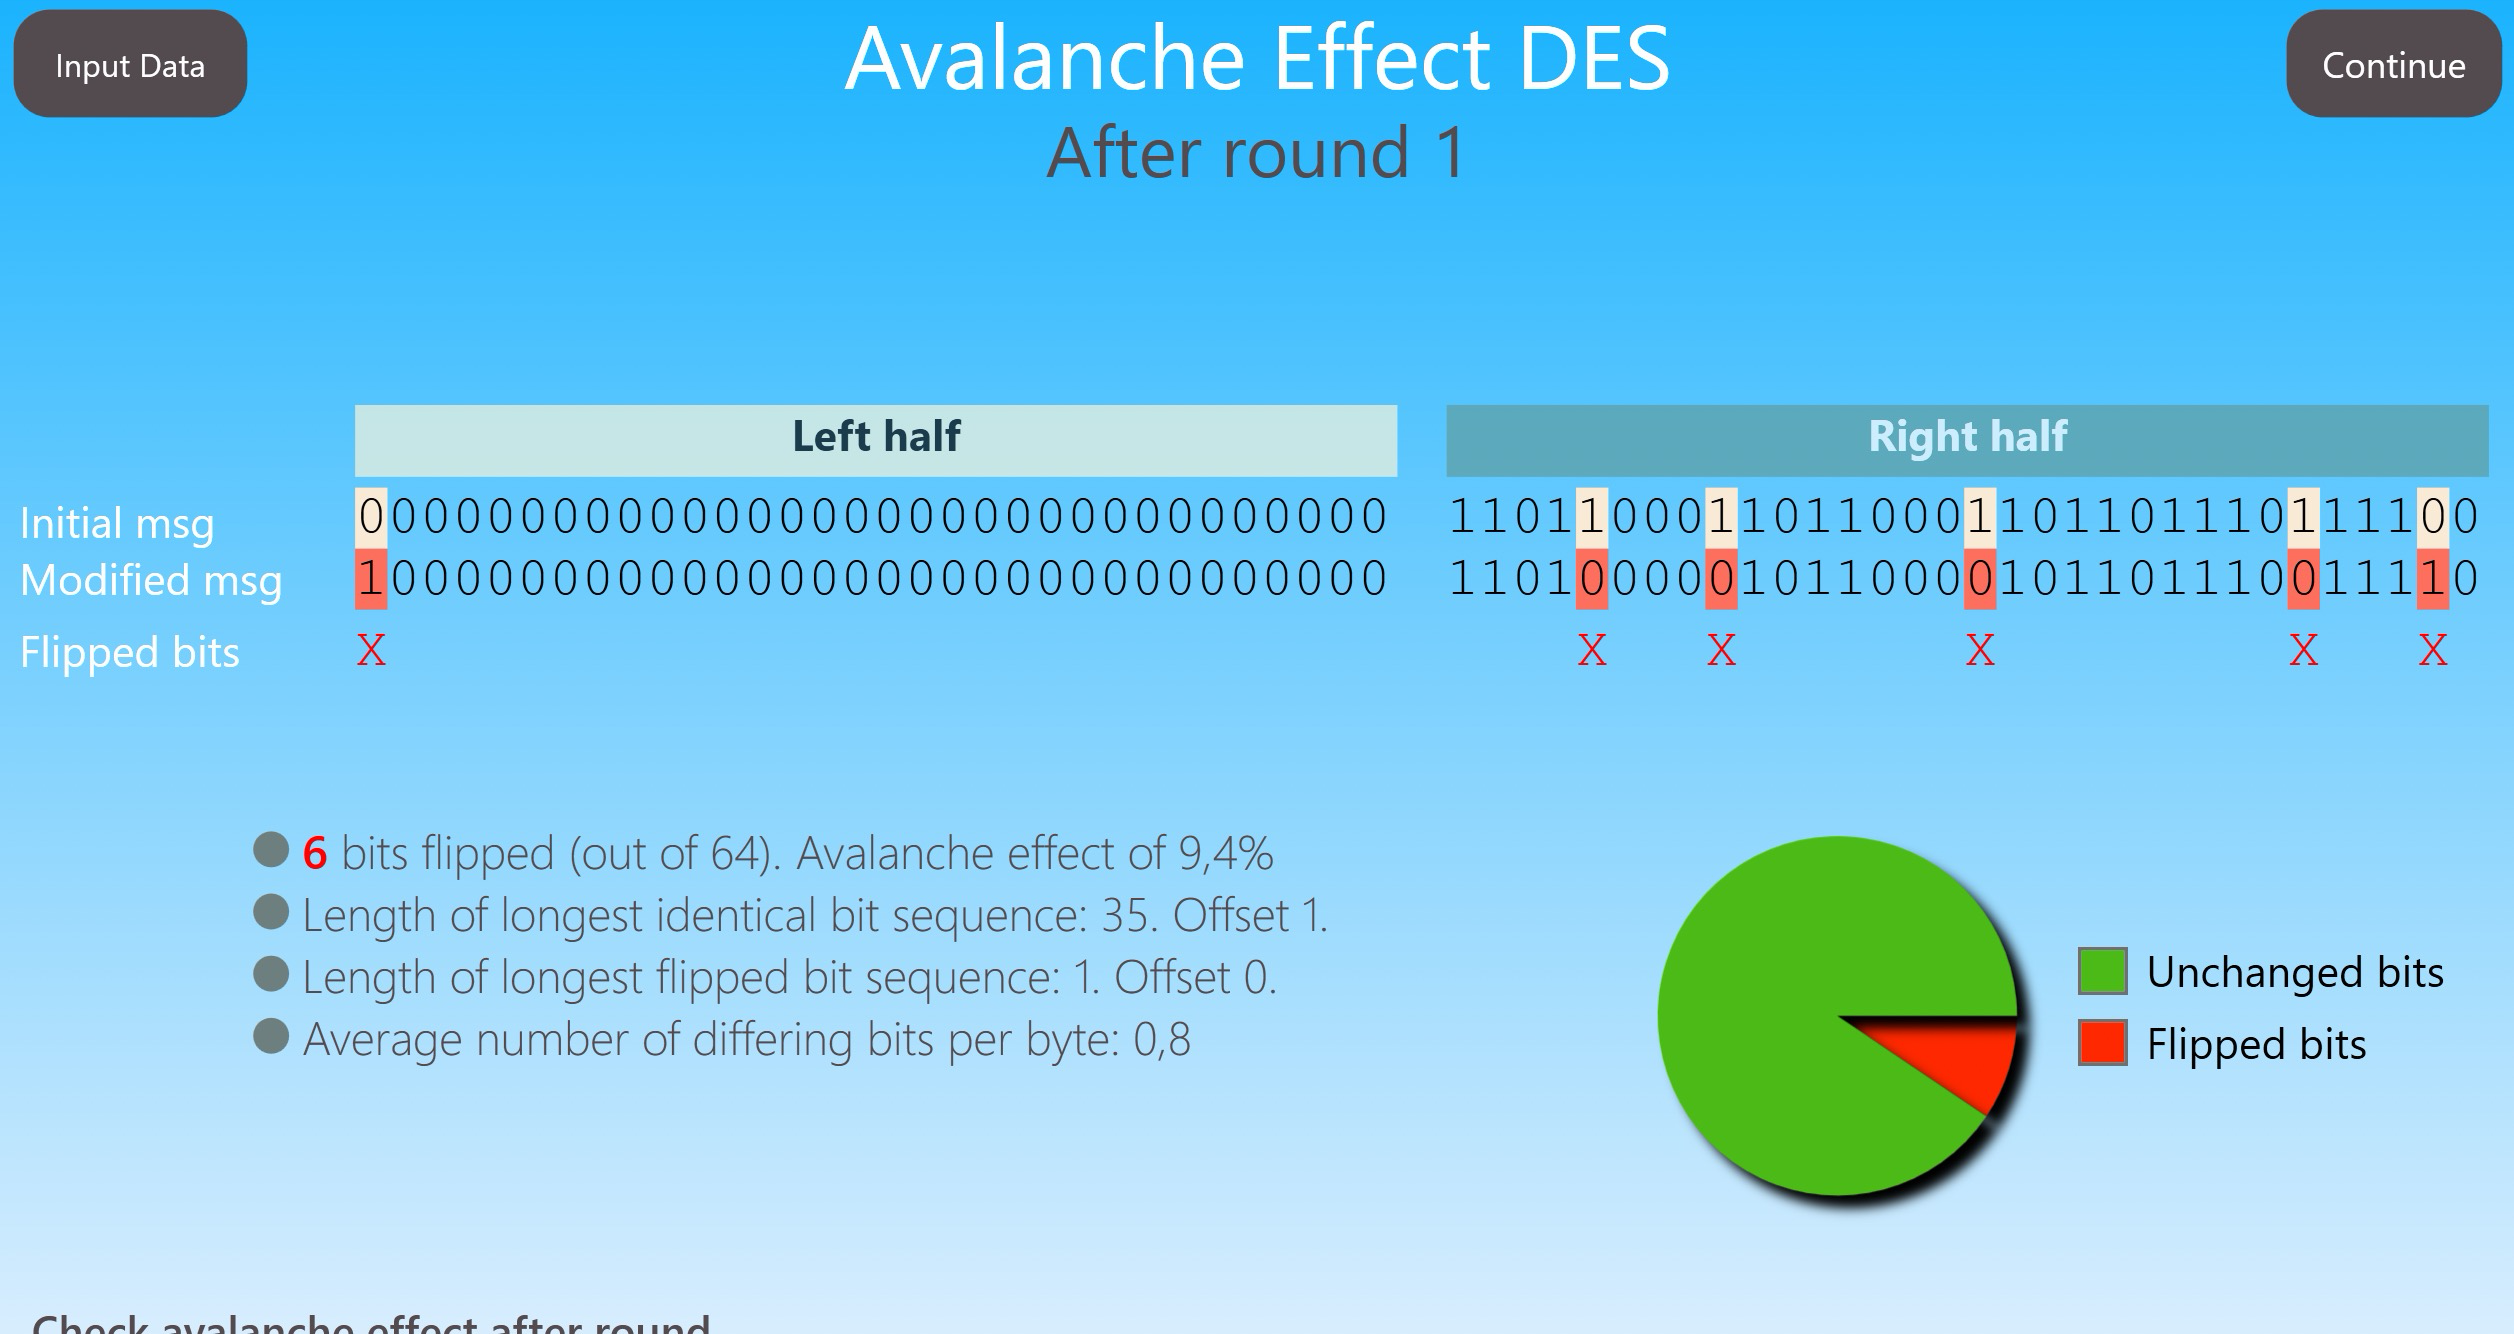
\includegraphics[scale=0.1]{image.png}
    \caption{DES Avalanche Effect Results}
    \label{fig:des-avalanche}
\end{figure}


\newpage
\section*{Appendix: Instructions for Homework Sheet Preparation in \LaTeX}

\subsection{How to Include an Image}
A picture can be included in your document using the \LaTeX code used to obtain Figure \ref{fig:demo}.

\begin{figure}
    \centering
    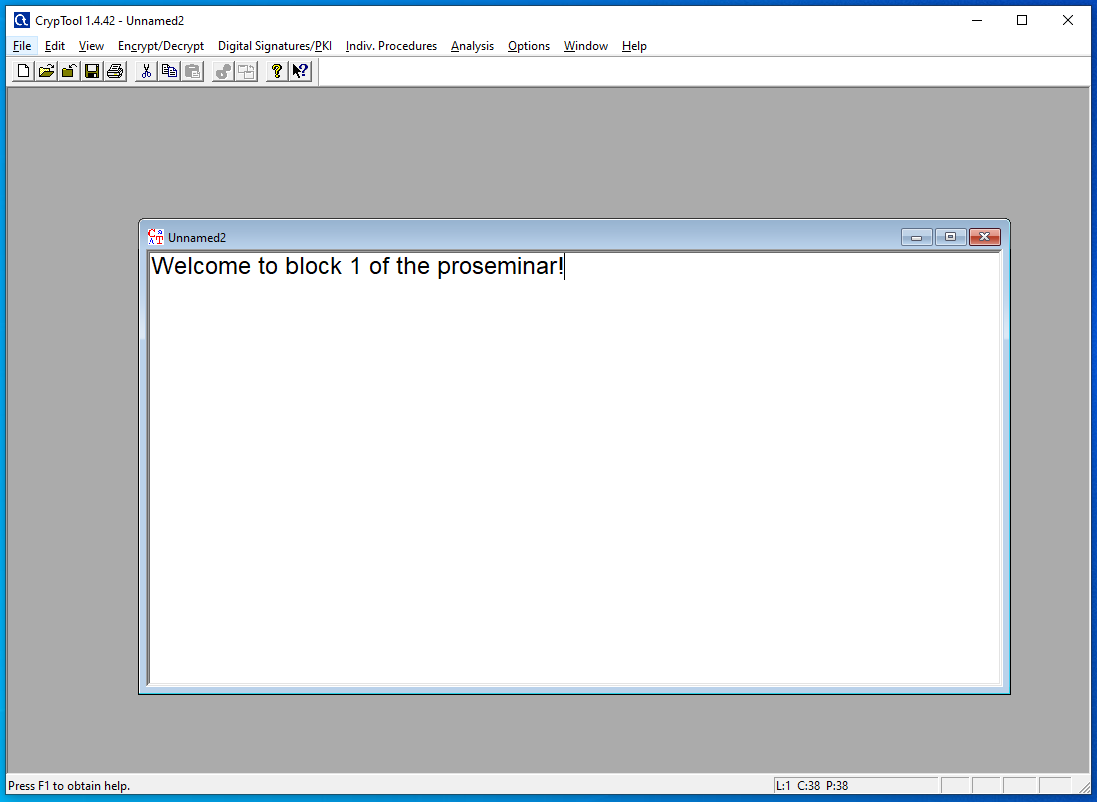
\includegraphics[scale=0.35]{figures/cryptool1.PNG}
    \caption{The code of this figure can be used when preparing your homework.}
    \label{fig:demo}
\end{figure}

\subsection{How to Include a Table}

A table can be included using the commands used to obtain Table \ref{tab:example}.

\begin{table}[ht]
    \centering
    \begin{tabular}{|c|c|c|}
    \hline
        Software & Assessment & Comments \\
        \hline
        Suite A & works well & internal use only \\
        \hline
        Suite B & freely usable & observe guidance document \\
        \hline
        Suite C & restricted & Requires compiler \\
        \hline 
    \end{tabular}
    \caption{Caption}
    \label{tab:example}
\end{table}

\subsection{How to List Data like Hexdumps}

Hexadecimal encoding provides a way to encode data in a machine and human-readable way. The code that has been used to generate Listing \ref{lst:example} can be used to include hex-data, including the one provided by \ctone{}. 
\begin{lstlisting}[style=plusStyle, caption={Example for how to include hex-data.},basicstyle=\tiny\ttfamily,label=lst:example]
50 63 D8 D0 D8 E4 FC F7 09 FB 1F 40 C1 99 E7 62 56 8A 20 77 B9 D6 F7 21 B3 61 F0 8D
96 AA 45 E3 A0 A5 11 97 58 17 2B 53 60 6D A3 2C A0 4C 2E 1F 5F 31 94 6A CC 09 28 8E
E0 0E 7C 23 2E 2F E3 E6 6A 02 AA D2 A7 41 80 6D AF 5D 72 63 0E AE A8 1F 3A 38 E3 91
74 56 B6 D7 59 C8 14 4B 0F C2 D8 9F 46 98 26 92 AF 5D 60 9E 5D AC 30 A1 DD 7A D1 95
49 AD 54 3C 93 B0 DF BC B2 57 83 AF F7 43 D8 98 0B 06 A4 6B 42 4C 8D 44 F4 7C BB B0
A6 B3 A2 7E 9C 11 D7 A6 98 23 EC 23 8E C8 AC FD 15 B0 2F 2B EC 49 25 B5 70 9C 0B D5
8A 24 5F 8C 7D 1A 32 E9 4C EF E7 B1 06 C7 D4 A2 C8 DA 01 15 99 E2 92 6B 0E DF 5B 36
15 2B 30 30 E0 5A A6 E0 80 2F 07 4F B4 4F 66 F8 17 A0 A3 72
\end{lstlisting}


\end{document}